\section{DVND}\label{subsec:dvnd}

Foi descrito na Seção~\ref{sec:dvndClassico} o algoritmo do DVND, contudo um modelo dataflow para o DVND pode ser visto na Figura\ref{fig:dvndGraph}, o método usa $P + 1$ nós iniciais (\textit{ini0}, \textit{ini1}, \dots \textit{iniP}) que alimentam os nós operadores (\textit{Swap, 2-Opt, OrOpt-1, OrOpt-2, OrOpt-3}) e o nó gerente (\textit{man}) com a solução inicial para a busca local.

\begin{figure}[htbp]
    \centerline{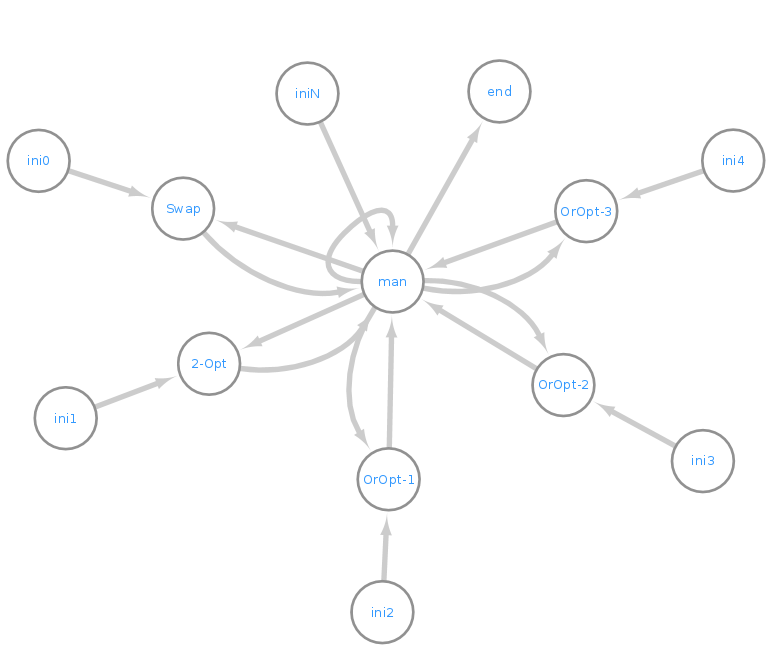
\includegraphics[scale=0.6]{figuras/dvnd/DVND_dataflow_nomes.png}}
    \caption{Arquitetura simplificada do dataflow para o DVND com as vizinhanças utilizadas.}
    \label{fig:dvndGraph}
\end{figure}

Cada nó operador utiliza uma estratégia de vizinhança diferente, quando termina de enumerar as soluções este retorna a melhor para o nó gerente que mantém a melhor solução encontrada até o momento.
Então o nó gerente identifica a melhor solução conhecida e a envia de volta para o dataflow (como no Algoritmo.~\ref{alg:dvndMan}) que encaminha a solução para todos os nós operadores parados, o processo se repete até que nenhum nó operador encontre uma solução melhor.
Então a melhor solução encontrada é enviada para o nó final (\textit{end}) que salva o resultado da busca local.

\begin{algorithm}[htpb]
\caption{Nó \textit{man} do DVND}
\label{alg:dvndMan}
\begin{algorithmic}[1]
    \Function{DVND\_Man}{Solução: s, Histórico: H}
        \Let{$H$}{$H \cup \{s\}$}
        \Return{$bestSolution(H)$}
    \EndFunction
\end{algorithmic}
\end{algorithm}

O critério de parada é alcançado quando nenhum nó operador consegue melhorar a solução atual significando que está corresponde a ótimo local para todas as vizinhanças usadas no processo.
Este é, de certa forma, o mesmo critério utilizado por ambos RVND e DVND, contudo o caminho percorrido pelos diferentes processos pode levar a a ótimos locais diferentes. Tanto para o RVND quanto DVND as estratégias de vizinhança são atribuídas aos nós \textit{oper} e os métodos não definem o comportamento interno destes nós facilitando sua alteração ou mesmo a adição de uma nova vizinhança.

\begin{figure}[htbp]
    \centerline{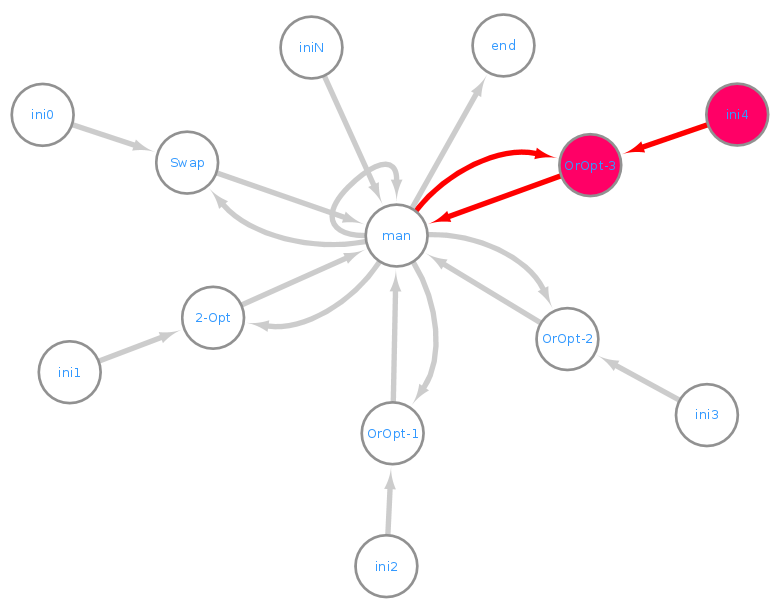
\includegraphics[scale=0.6]{figuras/dvnd/DVND_dataflow_nomesDestacado.png}}
    \caption{Uma vizinhança e suas ligações ao grafo dataflow no DVND.}
    \label{fig:dvndGraphDestacado}
\end{figure}

Como dito anteriormente, qualquer vizinhança pode ser facilmente acoplada ao procedimento apenas adicionando um novo nó operador \textit{oper} ao grafo dataflow, conforme destacado na Figura~\ref{fig:dvndGraphDestacado}, o que é uma grande característica do método, e como os nós são independentes é possível fazê-lo sem impactar nos outros nós.
Inicialmente pode parecer que muitos nós operadores podem sobrecarregar o nó gerente, mas é importante notar que o tempo computacional gasto pelos nós operadores é geralmente muito mais caro (exploração das vizinhanças é o processo mais caro de uma meta-heurística), desta forma não será um grande problema mesmo quando os nós operadores responderem em tempos curtos.

No trabalho apresentado em~\cite{df-dvnd2018} o modelo dataflow usado possuía apenas uma porta de saída então a mensagem seria enviada para todos os nós a ele vinculados, numa melhoria a esta implementação foi implementado e sugerido um aperfeiçoamento ao Sucuri para comportar portas de saída diferentes para destinos diferentes.
No modelo proposto (veja Figura~\ref{fig:dvndGraph}), o nó gerente é ligado a todos os nós operadores o que causaria uma inundação (\emph{flooding}) na rede, desta forma possuir mais de uma porta de saída permite evitar que um nó processe indevidamente uma solução ou que receba uma mensagem com uma indicação de que não deve ser processada o que causaria uma troca de mensagens desnecessária, problema esse que se intensifica ao rodar o processamento em rede.
Um problema que permanece é o escalonador centralizado, o que significa que num processamento em rede cada mensagem precisa ser enviada de volta para o computador rodando o nó gerente para só então ser enviada para o seu nó de destino, incluindo nisso as mensagens de \emph{feedback} explicadas no Sub-seção~\ref{text:flipFlop}.
Contudo a disponibilização de um escalonador distribuído demandaria um novo projeto para a o dataflow do DVND (Figura~\ref{fig:dvndGraph}) de forma a fazer melhor uso deste recurso.
Apesar das limitações atuais deste projeto em desenvolvimento, o Sucuri já provê um ambiente que pode ser facilmente escalado de uma máquina para um experimento em rede completamente distribuído.

\subsubsection{Passo iterativo}

Utilizando o termo convencionado na seção~\ref{subsec:passoIterativo}, cada passo iterativo do DVND retorna a melhor solução encontrada para todas as vizinhanças.
Dessa forma, sendo $N$ a união de todas as vizinhanças, o passo iterativo do DVND pode ser dado pela Equação~\ref{eq:dvndPassoIterativo}.
\begin{equation} \label{eq:dvndPassoIterativo}
\rho^{DVND}(s) = s' \in N \quad \textrm{com} \quad f(s') < f(s''), \forall s'' \in N(s) \land s'' \ne s
\end{equation}
Fazendo uso da notação de movimentos podemos escrever \ref{eq:dvndPassoIterativo} como a Equação~\ref{eq:dvndPassoIterativoMovimento}.
\begin{equation} \label{eq:dvndPassoIterativoMovimento}
\rho^{DVND}(s) = m \circ s\quad \textrm{com} \quad m \in \mathcal{M} \land \widehat{m} < \widehat{m_i} \mid \forall m_i \in \mathcal{M}
\end{equation}

Pelo passo iterativo do RVND $\rho^{RVND}$ (\ref{eq:rvndPassoIterativoMovimento}) e do DVND $\rho^{DVND}$ (\ref{eq:dvndPassoIterativoMovimento}) podemos concluir que $\rho^{DVND}(s) \le \rho^{RVND}(s)$, contudo isso não é suficiente para afirmar que o DVND encontre necessariamente melhores resultados.% pois o DVND pode acabar convergindo muito cedo para um mínimo local.

\subsection{Nó de flip flop}\label{subsec:flipFlop}

É esperado um comportamento sem estado para os nós num grafo de uma arquitetura dataflow contudo no modelo do DVND proposto (veja Figura~\ref{fig:dvndGraph}) o nó gerente precisa manter o histórico da melhor solução já encontrada até o momento e decidir se o método alcançou ou não um ótimo local. Para alcançar este comportamento, é apresentado em \cite{endm2018:araujo} um nó de flip flop \label{text:flipFlop} (nó \textit{FF} na Figura~\ref{fig:flipFlop}), este nó possui duas portas de entrada, uma que de fato recebe a informação do nó anterior e outra que o retro-alimenta com sua própria saída para manter o histórico do resultado. A intenção desse padrão é conceder ao nó a capacidade de realizar uma decisão baseada na última iteração sem necessariamente tornar o nó statefull.

\begin{figure}[htbp]
    \centerline{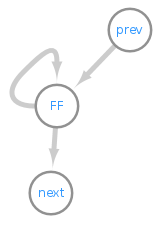
\includegraphics[scale=1.0]{figuras/dataflow/Flip_flop.png}}
    \caption{FF identifica o nó de flip flop.}
    \label{fig:flipFlop}
\end{figure}

É importante ressaltar que o nó \textit{oper0} no RVND (Figura~\ref{fig:rvndGraph}) também possui uma retroalimentação contudo não é um nó de flip flop pois não retroalimenta sua própria saída, este nó não precisa da informação de sua última execução para realizar o seu processamento, desta forma possui apenas uma porta de entrada.

\subsection{Múltiplas portas de saída}\label{subsec:multiplasSaidas}

Em modelo dataflow um nó será processado quando todas as suas dependências forem satisfeitas, contudo, ao final de seu processamento o resultado pode ser enviado como entrada para um ou mais nós.
Pode ser visto na Figura~\ref{fig:dataflowMo0} que o nó \textit{MO} está conectado a um nó com informação de entrada (nó \textit{prev}) e ligado a três nós de saída (\textit{next 0}, \textit{next 1} e \textit{next 2}).

\begin{figure}[htbp]
    \centerline{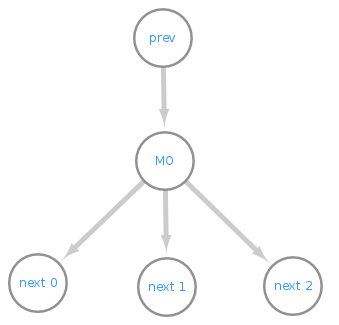
\includegraphics[scale=0.9]{figuras/dataflow/multi_output0.png}}
    \caption{Pedaço de um grafo dataflow em que o nó \textit{MO} do datalflow possui múltiplas saídas.}
    \label{fig:dataflowMo0}
\end{figure}

No modelo atual de implementação da biblioteca Sucuri é possível que um nó receba informações de vários outros nós contudo existe apenas uma porta de saída a qual podem estar conectados vários nós.

Pegando-se o exemplo da Figura~\ref{fig:dataflowMo3}, quando o nó \textit{MO} termina de processar seu resultado é enviado para a única porta de saída existente a qual estão ligados os nós \textit{next 0}, \textit{next 1} e \textit{next 2}, dessa forma todos os nós seguintes vão receber a informação e estarão aptos para processamento mesmo que a informação não seja destinada a eles.
Cada um desses nós terá então que verificar se a mensagem é destinada a ele antes de processar ou não a informação.

\begin{figure}[htbp]
    \centerline{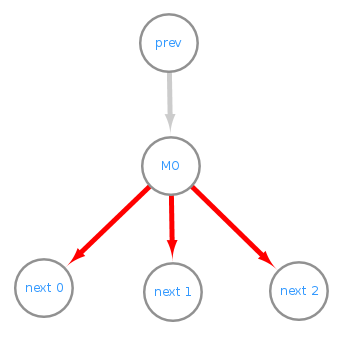
\includegraphics[scale=0.9]{figuras/dataflow/multi_output3.png}}
    \caption{Quando o nó \textit{MO} termina de processar seu resultado é enviado para todos os nós subsequentes (\textit{next 0}, \textit{next 1} e \textit{next 2}).}
    \label{fig:dataflowMo3}
\end{figure}

Foi implementada a alteração exemplificada na Figura~\ref{fig:dataflowMo1}, nesse caso existe uma porta de saída para cada nó ligado ao nó \textit{MO}, este identifica os destinatários da mensagem e aciona apenas aqueles necessários.

\begin{figure}[htbp]
    \centerline{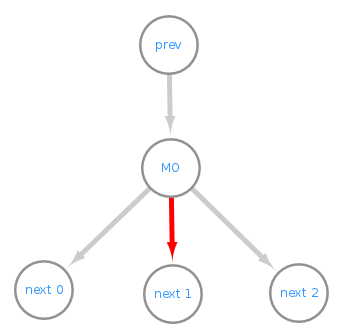
\includegraphics[scale=0.9]{figuras/dataflow/multi_output1.png}}
    \caption{Quando o nó \textit{MO} termina de processar é possível escolher qual porta de saída será utilizada e assim decidir o destino da informação.}
    \label{fig:dataflowMo1}
\end{figure}

No DVND, ao escolher o destinatário da mensagem é possível evitar uma grande quantidade de transmissões desnecessárias de mensagens, evitando assim que os nós de vizinhança sejam acionados apenas para identificar que não precisam processar a mensagem.
Vejamos, por exemplo, o nó \textit{man} da Figura~\ref{fig:dvndGraph} sem o artifício de múltiplas portas de saída todas as mensagens serão enviadas para todas as 5 vizinhanças e para o nó finalizador (\textit{end}) sendo que a mensagem só é enviada para os nós ociosos naquele momento.

A implementação de múltiplas portas de saída trás vantagens ainda mais significativas quando o tamanho da mensagem a ser transmitido é grande e quando a execução do processamento está sendo feita em um ambiente de mais de uma máquina o que envolve troca de mensagens pela rede.
